% To generate PDF, type ./run flashNorm

\documentclass{article}
\usepackage{arxiv}
\usepackage[numbers]{natbib} % for author-year citation style: \usepackage{natbib}
\numberwithin{equation}{section} % numbering of equations as 2.1 (for section 2, equation 1)

% shortcuts
\newcommand{\mat}[1]{\mathbf{#1}}     % shortcut for matrix
\newcommand{\RMS}[1]{\text{RMS}(#1)}  % shortcut for RMS(x)
\def\rms{\text{RMS}(\vec{a})}         % RMS(a)
\def\f1n{\frac{1}{n}}                 % 1/n
\def\sas{\sum_{i=1}^n a_i^2}          % sum over a_i squared
\def\W*{\mat{W}^\ast}                 % matrix W*
\def\a{\vec{a}}                       % vector a
\def\b{\vec{b}}                       % vector b
\def\c{\vec{c}}                       % vector c

\title{Transformer tricks: Flash normalization [work in progress]}

\author{Nils Graef, Matthew Clapp, TBD \\
  \href{https://openmachine.ai}{OpenMachine}, San Francisco Bay Area, \texttt{info@openmachine.ai}}

\begin{document} \maketitle

\begin{abstract}
RMSNorm \citep{rms} is used by many LLMs such as Llama, Mistral, and Gemma \citep{LLaMA, mistral, gemma}. As noted in \citep{openelm}, RMSNorm can be a bottleneck. Therefore, this paper details FlashNorm, which is an exact but faster implementation of RMSNorm followed by linear layers. See \citep{tricks, remove, precompute} for code and more transformer tricks.
\end{abstract}

\section{Flash normalization}
RMSNorm \citep{rms} normalizes the elements  $a_i$ of vector $\a$ as $y_i = \frac{a_i}{\rms} \cdot g_i$ with $\rms = \sqrt{\f1n \sas}$ and normalization weights $g_i$. In transformer \citep{vanilla} and other neural networks, RMSNorm is often followed by a linear layers as illustrated in Fig. \ref{fig1}(a), which we optimize as follows:
\begin{itemize}[topsep=-1pt, itemsep=-1pt]
  \item \textbf{Weightless normalization}: We merge the normalization weights $g_i$ into the linear layer with weights $\mat{W}$, resulting in a modified weight matrix $\W*$ with $W_{i,j}^\ast = g_i \cdot W_{i,j}$ as illustrated in Fig. \ref{fig1}(b).
  \item \textbf{Deferred normalization}: Instead of normalizing before the linear layer, we normalize after the linear layer, as shown in Fig. \ref{fig1}(c). This only works if the linear layer is bias-free, which is the case for many LLMs such as Llama, Mistral, and Gemma.
\end{itemize}

\begin{figure}[h!] \centering  % the [h!] tries to place the picture right here
  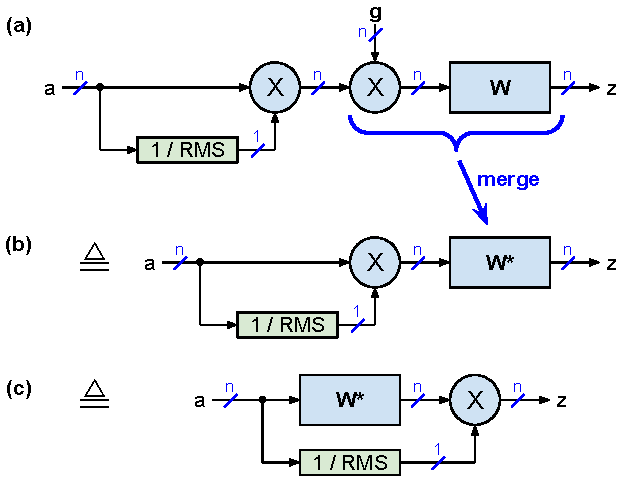
\includegraphics[scale=1.0]{figs/flash_fig1.pdf}
  \caption{Mathematically identical implementations of RMSNorm followed by a bias-free linear layer: (a) unoptimized version with weight matrix $\mat{W}$; (b) optimized version with normalization weights $g_i$ merged into the linear layer with new weights $\W*$; (c) optimized version with deferred normalization.}
\label{fig1} \end{figure}

In summary, FlashNorm eliminates the normalization weights and defers the normalization to the output of the linear layer, which removes the bottleneck described at the end of this paper. Deferring the normalization is similar to Flash Attention \citep{flash-attention}, where the normalization by the softmax denominator is done \emph{after} the multiplication of softmax arguments with value projections (V) (so that keys and values can be processd in \emph{parallel}). Therefore, we call our implementation \emph{flash} normalization (or FlashNorm), which allows us to compute the linear layer and $\rms$ in \emph{parallel}.

\citeauthor{openelm} report significant changes in the overall tokens-per-second throughput when they modify the layer normalization implementation, which they attribute to a lack of kernel fusion for the underlying GPU. The simplifications presented here reduce the number of operations and thus the number of the individual kernel launches mentioned in \citep{openelm}.

\section{Flash normalization for FFN}
For the feed-forward networks (FFN) of LLMs, the linear layers at the FFN input usually have more output channels than input channels. In this case, deferring the normalization requires more scaling operations (i.e. more multiplications). This section details ways to reduce the number of scaling operations for bias-free FFNs.

\subsection{Flash normalization for FFNs with ReLU}
Even though ReLU is a nonlinear function, multiplying its argument by a non-negative scaling factor $s$ is the same as scaling its output by $s$, i.e. $\text{ReLU}(s \cdot \a) = s \cdot \text{ReLU}(\a)$ for $s \ge 0$ \citep{ReLU}. Because of this scale-invariance, we can defer the normalization to the output of the FFN as illustrated in Fig. \ref{fig2}(b), which saves $f - n$ multipliers.

\begin{figure}[h!] \centering
  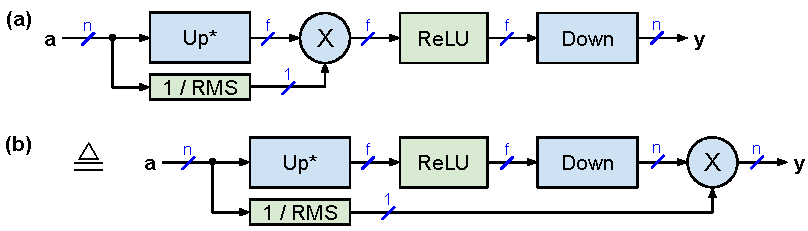
\includegraphics[scale=1.0]{figs/flash_fig2.pdf}
  \caption{FFN with ReLU and preceding flash normalization: (a) unoptimized version; (b) optimized version where the normalization is deferred to the output of the FFN. Up and Down denote the linear layers for up and down projections.}
\label{fig2} \end{figure}

\subsection{Flash normalization for FFNs with GLU variant}
Fig. \ref{fig3}(a) shows an FFN with a GLU variant \citep{GLU} and flash normalization at its input. The flash normalization requires two sets of $f$ multipliers at the outputs of the Gate and Up linear layers in Fig. \ref{fig3}(a). One set can be deferred to the FFN output in Fig. \ref{fig3}(b), which saves $f - n$ multipliers.

\begin{figure}[h!] \centering
  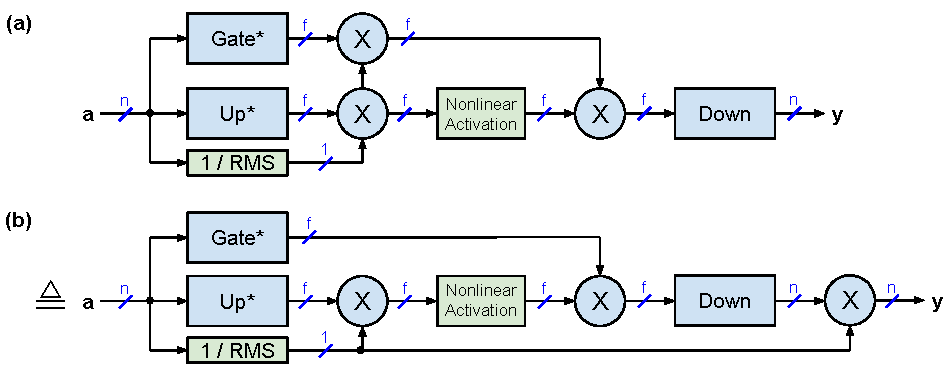
\includegraphics[scale=1.0]{figs/flash_fig3.pdf}
  \caption{FFN with GLU variant and preceding flash normalization: (a) unoptimized version; (b) optimized version with fewer scaling multipliers. Gate, Up, and Down denote the linear layers for gate, up, and down projections.}
\label{fig3} \end{figure}

\textbf{Special case for ReGLU and Bilinear GLU}: If the activation function is ReLU (aka ReGLU \citep{GLU}) or just linear (aka bilinear GLU \citep{GLU}), then we can also eliminate the scaling before the activation function and combine it with the scaling at the output as illustrated in Fig. \ref{fig4}(b), which saves $2f - n$ multipliers. Now the output scaling is using the reciprocal of the squared RMS as scaling value, which is the same as the reciprocal of the mean-square (MS):
\begin{equation*}
  \frac{1}{(\rms)^2} = \frac{1}{\text{MS}(\a)}
  = \frac{1}{\f1n \sas} = \frac{n}{\sas}
\end{equation*}

\begin{figure}[h!] \centering
  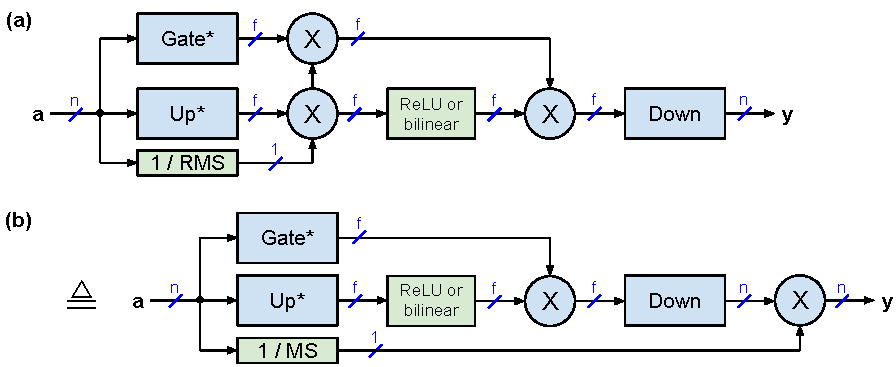
\includegraphics[scale=1.0]{figs/flash_fig4.pdf}
  \caption{FFN with ReGLU (or bilinear GLU) and preceding flash normalization: (a) unoptimized version; (b) optimized version with fewer scaling multipliers.}
\label{fig4} \end{figure}

\section{Flash normalization for attention with RoPE}
\begin{figure}[h!] \centering
  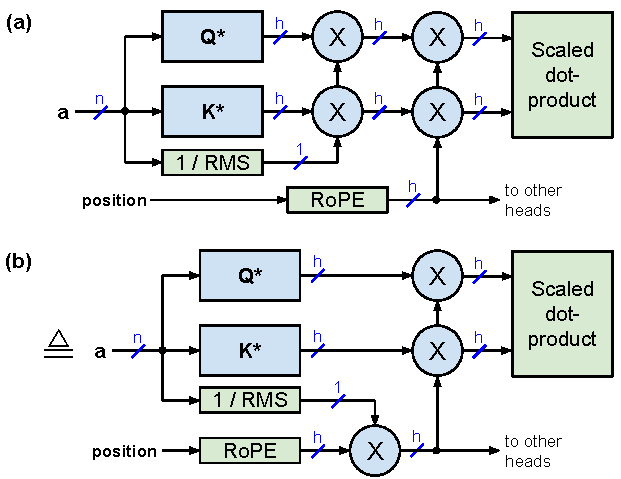
\includegraphics[scale=1.0]{figs/flash_fig5.pdf}
  \caption{Flash normalization for scaled dot-product attention with RoPE: (a) unoptimized version; (b) optimized version where the normalization is fused with RoPE.}
\label{fig5} \end{figure}

Fig. \ref{fig5}(a) shows the Q and K linear layers with flash normalization followed by RoPE \citep{RoPE} and scaled dot-product attention \citep{vanilla}:
\begin{itemize}[topsep=-1pt, itemsep=-1pt]
  \item Q* and K* are the linear layers for Q (queries) and K (keys) fused with the normalization weights of the activation vector $\a$ (according to flash normalization).
  \item $h$ is the dimension of the attention heads.
  \item Note that the RoPE scaling vector only depends on the position of activation vector $\a$ and is shared among all attention heads. Therefore, it’s more efficient to first scale the RoPE scaling vector by $1/ \rms$ and then share this fused scaling vector among all attention heads as illustrated in Fig. \ref{fig5}(b). This saves $h \cdot (H - 1)$ multipliers, where $H$ is the number of attention heads.
  \item Furthermore, we can fuse the scaling factor $1/ \sqrt{h}$ of the scaled dot-product with the $1/ \rms$ factor (note that we need to use $\sqrt{1/ \sqrt{h}}$ as a scaling factor for this).
  \item Unfortunately, the V linear layer (value projection) still needs the normalization at its output.
\end{itemize}

\section{Optimizations for QK-normalization with RoPE}
Some LLMs use query-key normalization \citep{QKnorm}. For example, each layer of OpenELM \citep{openelm} has the following two sets of normalization weights:
\begin{itemize}[topsep=-1pt, itemsep=-1pt]
  \item \verb+q_norm_weight+: query normalization weights for all heads of this layer
  \item \verb+k_norm_weight+: key normalization weights for all heads of this layer
\end{itemize}
Unfortunately, FlashNorm can't be applied for QK-normalization. But for the type of QK-normalization used in OpenELM, we can apply the following two optimizations detailed in the next sections:
\begin{enumerate}[topsep=-1pt, itemsep=-1pt]
  \item Eliminate the RMS calculation before the Q and K linear layers.
  \item Fuse the normalization weights with RoPE.
\end{enumerate}

\subsection{Eliminate RMS calculation before QK linear layers}
Fig. \ref{fig6}(a) shows a linear layer with flash normalization followed by QK-normalization. The weights of the first normalization are already merged into the linear layer weights $\W*$. Note that $\RMS{s \cdot \a} = s \cdot \rms$ where $s$ is scalar and $\a$ is a vector. Due to this scale-invariance of the RMS function, the second multiplier (scaler $s_c$) in the pipeline of Fig. \ref{fig6}(a) cancels out the first multiplier (scaler $s_b$). Fig. \ref{fig6}(b) takes advantage of this property. We can express this by using the vectors $\a, \b, \c$ along the datapath in Fig. \ref{fig6} as follows:
\begin{itemize}[topsep=-1pt, itemsep=-1pt]
  \item Note that $s_c = \frac{1}{\RMS{\c}} = \frac{1}{\RMS{\b \cdot s_a}} = \frac{1}{s_a \cdot \RMS{\b}} = \frac{s_b}{s_a}$.
  \item With above, we can show that the $y$ outputs of figures \ref{fig6}(a) and \ref{fig6}(b) are identical:
    \begin{equation*}
      y = \a \cdot \W* \cdot s_a \cdot s_c \cdot \vec{g} = \a \cdot \W* \cdot s_a \cdot \frac{s_b}{s_a} \cdot \vec{g}
      = \a \cdot \W* \cdot s_b \cdot \vec{g}
    \end{equation*}
\end{itemize}

\begin{figure}[h!] \centering
  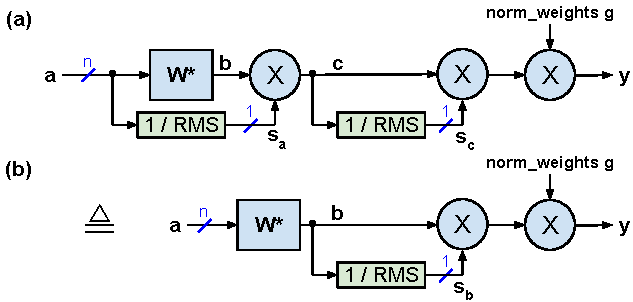
\includegraphics[scale=1.0]{figs/flash_fig6.pdf}
  \caption{Linear layer with flash normalization followed by another normalization: (a) unoptimized version; (b) optimized version.}
\label{fig6} \end{figure}

The scale-invariance property of $\rms$ doesn’t hold exactly true for RMS with epsilon (see appendix). This should not matter because the epsilon only makes an impact if the RMS (or energy) of the activation vector is very small, in which case the epsilon limits the upscaling of this low-energy activation vector.

\subsection{Fuse normalization weights with RoPE}
Fig. \ref{fig7}(a) illustrates QK-normalization with RoPE. If the QK-normalization weights are the same for all heads of a layer, as is the case for OpenELM \citep{openelm}, then we can fuse them with RoPE: multiply the RoPE scaling vector with the normalization weights and then share the fused scaling vectors across all heads of the LLM layer as shown in Fig. \ref{fig7}(b).

\begin{figure}[h!] \centering
  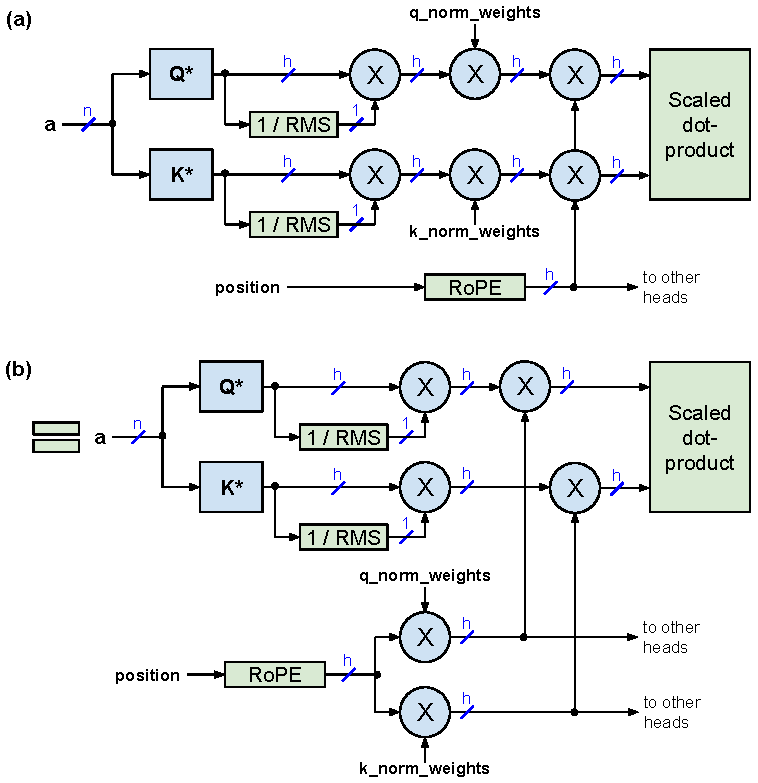
\includegraphics[scale=1.0]{figs/flash_fig7.pdf}
  \caption{QK-normalization with RoPE: (a) unoptimized version; (b) optimized version.}
\label{fig7} \end{figure}

\section{Bottleneck of RMS normalization for batch 1}
This section describes the compute bottleneck of RMS normalization that exists for batch size 1. This bottleneck is different from the bottleneck detailed in \citep{openelm}. Let’s consider a processor that has one vector unit and one matrix unit:

\begin{itemize}[topsep=-1pt, itemsep=-1pt]
  \item The matrix multiplications of the linear layers are performed by the matrix unit, while the vector unit performs vector-wise operations such as RMSNorm and FlashNorm.
  \item Let’s assume that the vector unit can perform $m$ operations per cycle and the matrix unit can perform $m^2$ operations per cycle, where $m$ is the processor width. Specifically:
  \begin{itemize}[topsep=-1pt, itemsep=-1pt]
    \item Multiplying an $n$-element vector with an $n \times n$ matrix takes $n^2$ MAD (multiply-add) operations, which takes $n^2/m^2$ cycles with our matrix unit.
    \item Calculating $1/\rms$ takes $n$ MAD operations (for squaring and adding) plus 3 scalar operations (for $1 / \sqrt{x/n}$), which takes $n/m$ cycles with our vector unit if we ignore the 3 scalar operations for simplicity.
    \item Scaling an $n$-element vector by a scaling factor takes $n$ multiply operations, which takes $n/m$ cycles.
  \end{itemize}
\end{itemize}

For the example $n = 512, m = 128$ and batch 1, Fig. \ref{fig8} shows timing diagrams without and with deferred normalization:
\begin{itemize}[topsep=-1pt, itemsep=-1pt]
  \item Without deferred normalization, the matrix unit has to wait for 8 cycles until the vector unit has calculated the RMS value and completed the scaling by $1/ \rms$ as illustrated in Fig. \ref{fig8}(a).
  \item As shown in Fig. \ref{fig8}(b), it is possible to start the matrix unit 3 cycles earlier if the weight matrix $\mat{W}$ is processed in row-major order for example. But the RMS calculation still presents a bottleneck.
  \item FlashNorm eliminates this bottleneck: With deferred normalization, the matrix unit computes the vector-matrix multiplication in parallel to the vector unit's RMS calculation as shown in Fig. \ref{fig8}(c). The scaling at the end can be performed in parallel to the matrix unit if $\mat{W}$ is processed in column-major order for example.
\end{itemize}

\begin{figure}[h!] \centering
  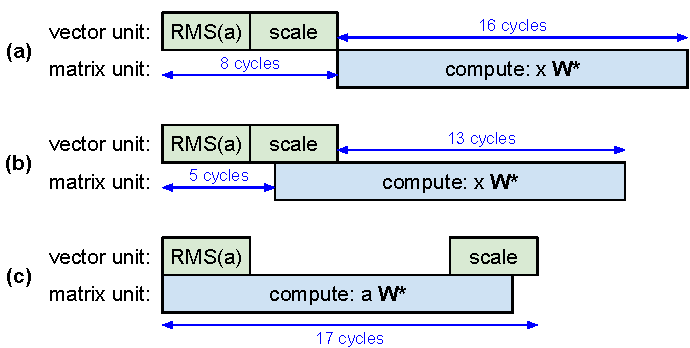
\includegraphics[scale=1.0]{figs/flash_fig8.pdf}
  \caption{Timing diagrams for $n = 512, m = 128$: (a) without deferred normalization; (b) with interleaved normalization and vector-matrix multiplication; (c) with deferred normalization.}
\label{fig8} \end{figure}

\section{Experiments}
Refer to \cite{tricks} for Python code that demonstrates the mathematical equivalency of the optimizations presented in this paper.
TODO: Modify OpenELM and/or Llama and show the speedup, add a TPS report (tokens-per-second).

\section{Future work}
Future work should investigate which of the presented optimizations are applicable for speeding up training of LLMs.

\bibliographystyle{unsrtnat}
\bibliography{references}

\section*{Appendix}

\subsection*{RMS with epsilon}
Many implementations add a small epsilon $\epsilon$ to the RMS value to limit the resulting scaling factor $1/\rms$ and to avoid division by 0 as follows:
\begin{equation*}
 \text{RMSe}(\a) = \sqrt{\epsilon + \f1n \sas} = \sqrt{\epsilon + \left( \rms \right)^2}
\end{equation*}

$\text{RMSe}(\a)$ can be used as a drop-in-replacement for RMS. The popular HuggingFace transformer library calls this epsilon \verb+rms_norm_eps+, which is set to $10^{-5}$ for Llama3.

\subsection*{Eliminating $1/n$}
This section details a small optimization that eliminates the constant term $1/n$ from the RMS calculation. First, we factor out $1/n$ as follows:
\begin{equation*}
  \rms = \sqrt{\f1n \sas} = \sqrt{\f1n} \sqrt{\sas} = \sqrt{\f1n} \cdot \text{RSS}(\a)
\end{equation*}
where we define the function RSS (Root Squared Sum) as
\begin{equation*}
  \text{RSS}(\a) = \sqrt{\sas}
\end{equation*}

We can now merge the constant term into the normalization weights $g_i$ as follows:
\begin{equation*}
  y_i = \frac{a_i}{\rms} \cdot g_i =
  \frac{a_i}{\text{RSS}(\a)} \sqrt{n} \cdot g_i =
  \frac{a_i}{\text{RSS}(\a)}          \cdot g_i^\ast
\end{equation*}
with new normalization weights $g_i^\ast = \sqrt{n} \cdot g_i$ . These new normalization weights can now be merged with the weights $\mat{W}$ of the following linear layer as shown in the previous sections. This optimization also applies for the case where we add an epsilon as detailed in the previous section. In this case, we factor out $1/n$ as follows:
\begin{equation*}
  \text{RMSe}(\a) = \sqrt{\epsilon + \f1n \sas}
  = \sqrt{\f1n \left( n \epsilon + \sas \right)}
  %= \sqrt{\f1n} \sqrt{n \epsilon + \sas}
  = \sqrt{\f1n} \cdot \text{RSSe}(\a)
\end{equation*}
where we define the function $\text{RSSe}(\a)$ as
\begin{equation*}
  \text{RSSe}(\a) = \sqrt{n \epsilon + \sas}
\end{equation*}

\end{document}
